%part of testing, cleaning and commissioning section

\subsection{Operational Procedure}
After the testing and commissioning CALIS has been installed inside CRH... 

Well, there also have been test deployments before that.
\subsubsection{Source Insertion}

\subsubsection{3 special positions}
home position or parking position - gate valve closed. The 

center of the TPC.

Full extension position - length of the cable.


\subsubsection{Vacuum evacuation (flushing) and nitrogen purging}
   One of the most important features of this system is making sure that the TMB and PC residue on the device are extracted from CALIS III prior to opening access ports to exchnage source or arms. This is  important for  safe working level of the people involved and for the detector.  This can be addressed through a system evacuation and nitrogen purge.  To accelerate the removal of the TMB in the scintillator fluid residue that is left after a deployment, CALIS III will undergo an evacuation with a vacuum pump. By lowering the pressure inside of CALIS below the vapor pressure of the TMB, it will cause the TMB to outgas and be removed through the vent line of the vacuum pump. An additional step to remove the TMB is to purge using N$_{2}$.  We will need to limit the potential flow rate of the nitrogen to ensure that an ODH (Oxygen Deficiency Hazard) condition is avoided in CRH.  Only once this is accomplished, will the view port be allowed to be opened and the source handled.     
  
The entire CALIS III  has been tested at FNAL  to hold pressure.  The system will be tested again after installation on the gate valve.
 

\begin{figure}[htbp]
 \centering
  \includegraphics[width=0.49\textwidth]{Figures/GasSystem.png}
  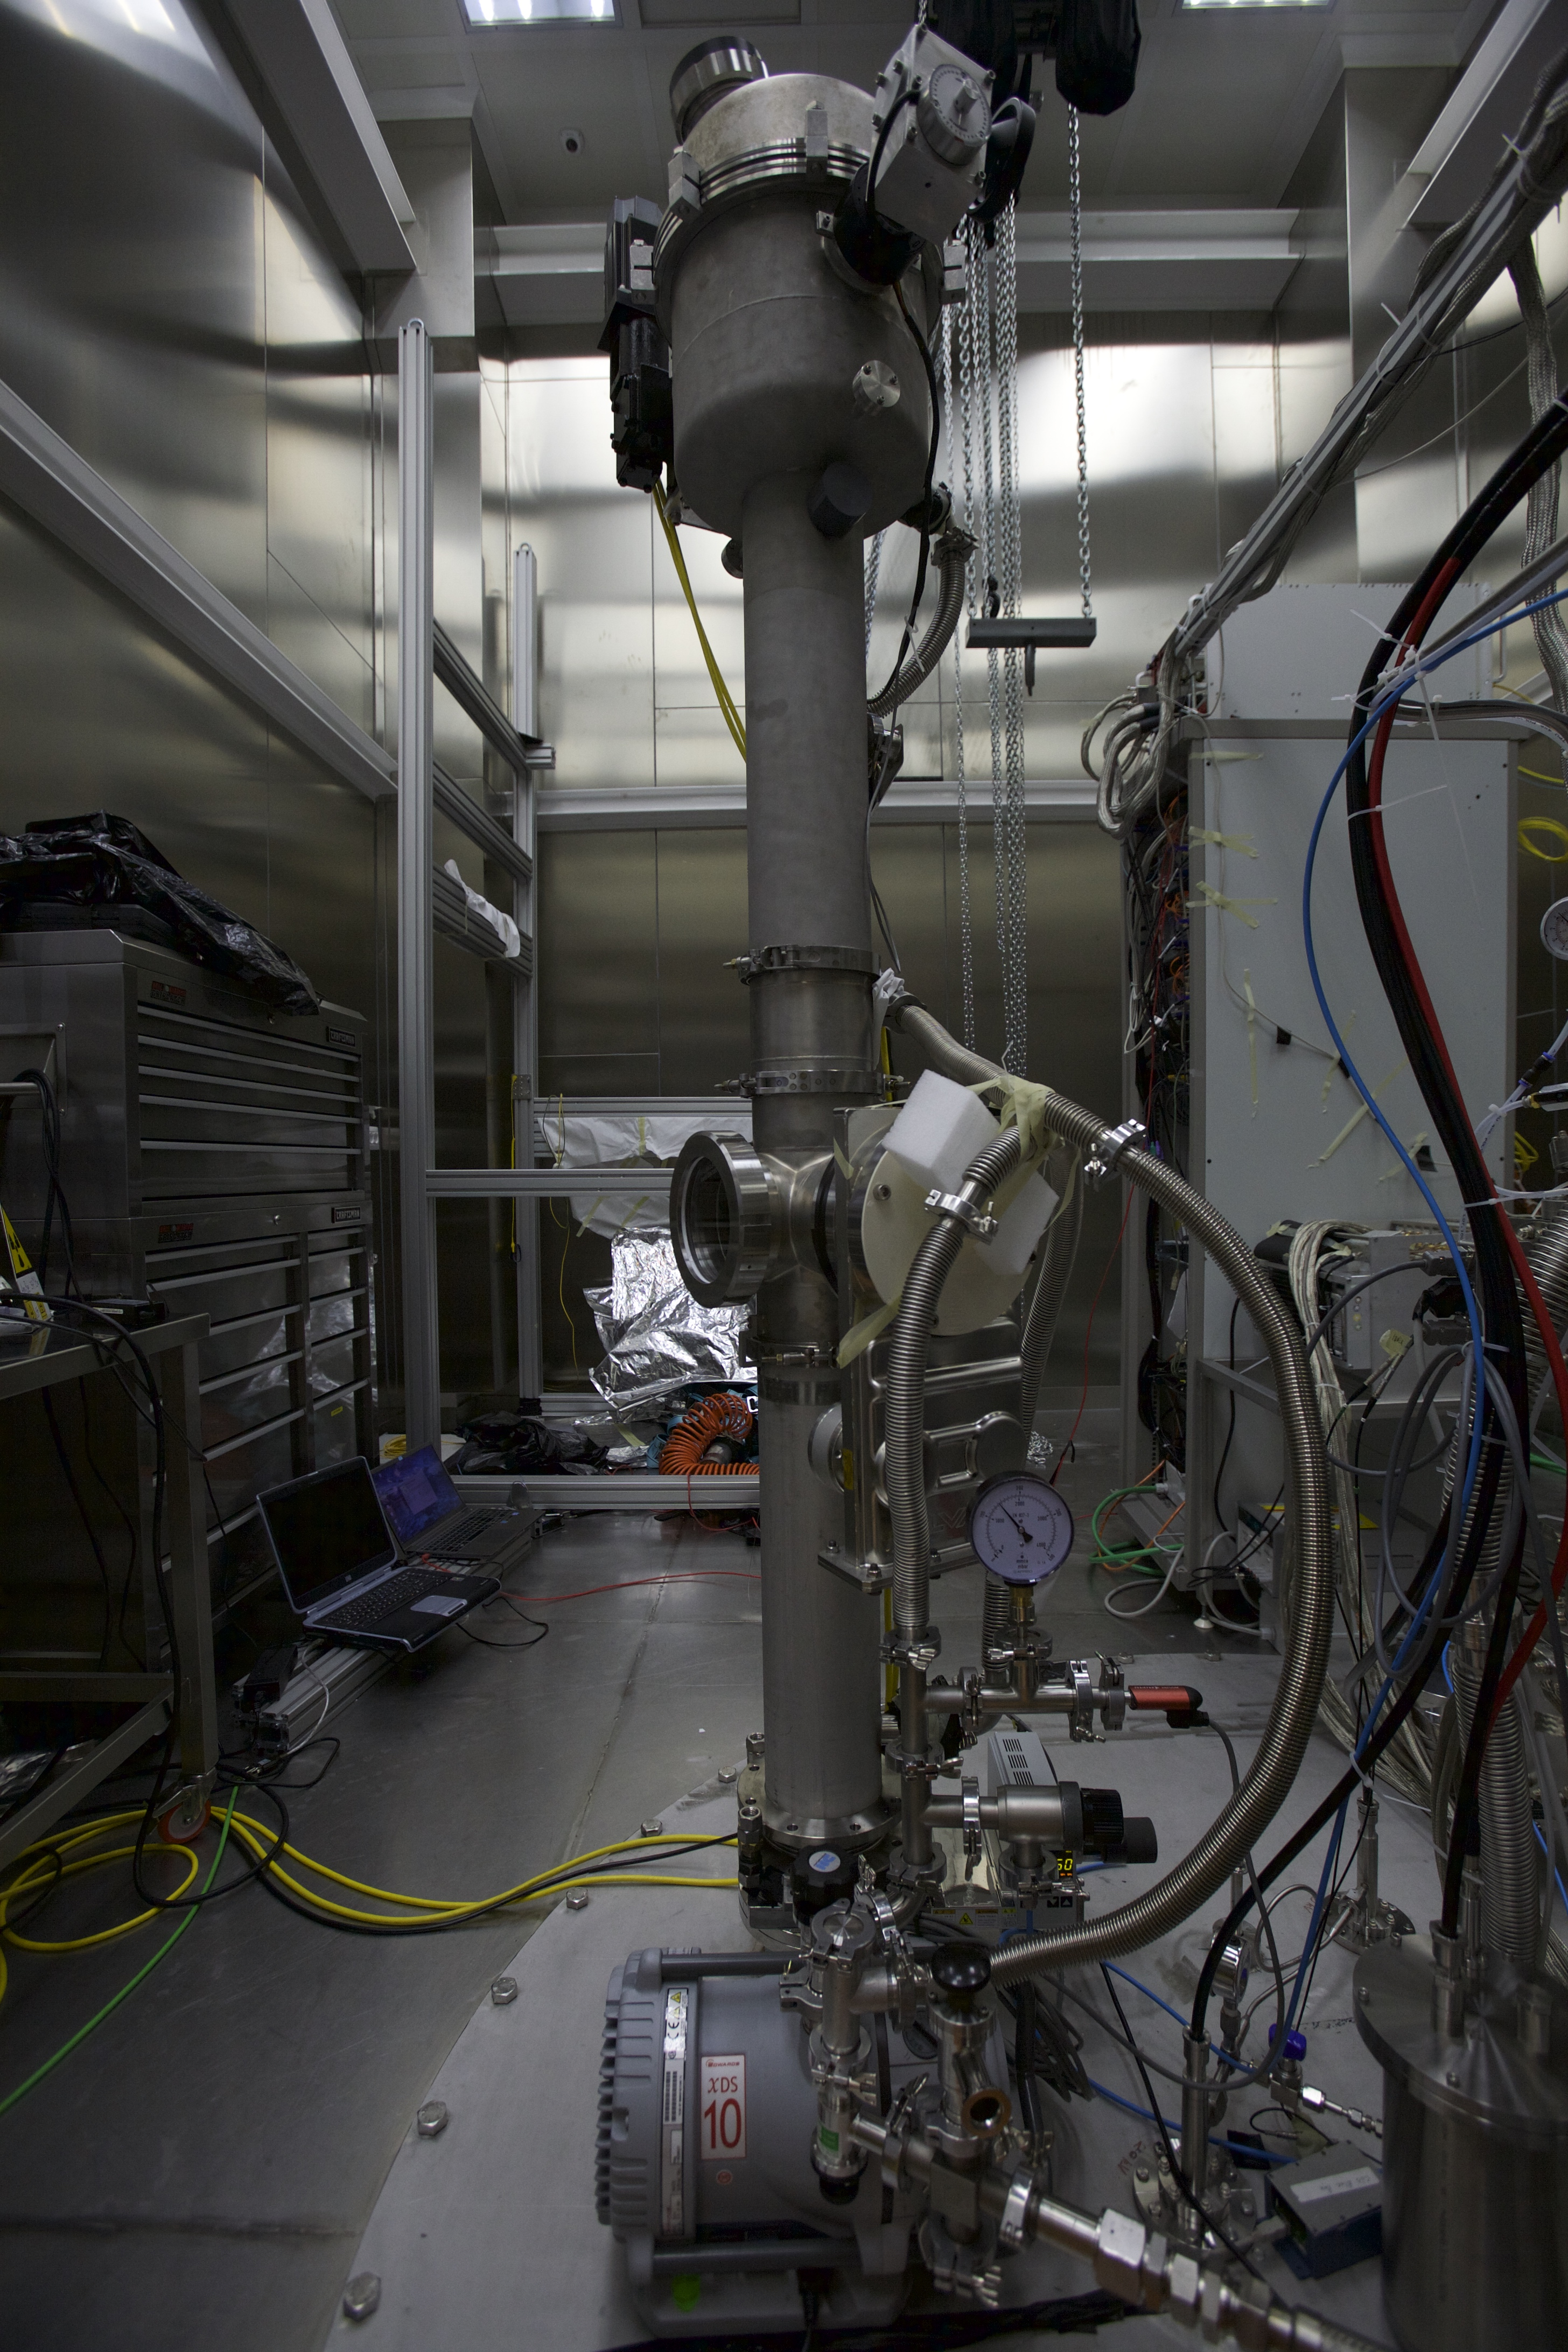
\includegraphics[width=0.49\textwidth]{Figures/CALIS_Tubings_IMG_3763.JPG}
  \caption{flushing and nitrogen purging system.}
  \label{fig:flushing_purging}
\end{figure}




\paragraph{Opening the Gate Valve}
\subsubsection{Positioning of Source}
\paragraph{Contact with Cryostat}
\paragraph{Cameras}
\subsubsection{Source Retraction and Extraction}
The source may not get in contact with the liquid scintillator. It is therefore sealed during the deployment in a dedicated source holder. In order to exchange sources the source arm and source holder has to be extracted from the pig into CRH and thereby comes in contact with normal air, containing oxygen and traces of water. After insertion a flush \& purge cycle is used to reduce, as known from glove boxes. No glove box present. Much more compact design.
% no glove box

After each deployment check that there is no leakage of Scintillator inside the source holder.



for what is helium leak tightness necessary? What was tested for helium leak tightness.



%tested for helium leak tightness

